%%%%%%%%%%%%%%%%%%%%%%%%%%%%%%%%%%%%%%%%%%%%%%%%%%%%%%%%%%%
% EPFL report package, main thesis file
% Goal: provide formatting for theses and project reports
% Author: Mathias Payer <mathias.payer@epfl.ch>
%
% To avoid any implication, this template is released into the
% public domain / CC0, whatever is most convenient for the author
% using this template.
%
%%%%%%%%%%%%%%%%%%%%%%%%%%%%%%%%%%%%%%%%%%%%%%%%%%%%%%%%%%%
\documentclass[a4paper,11pt,oneside]{report}
% Options: MScThesis, BScThesis, MScProject, BScProject
\usepackage[BScThesis]{EPFLreport}
\usepackage{xspace}
\usepackage{comments}
\usepackage{hyperref}
\usepackage{amsmath,amsthm,amssymb}
\usepackage{algpseudocode}
\usepackage{algorithm}
\usepackage{xcolor}
\usepackage{ stmaryrd } % for lightning symbol \lightning
\usepackage{graphicx} % for figures
\usepackage{wrapfig} 
\usepackage{subcaption} 
\usepackage{cleveref}

% define counters for theorems and lemmas
\newtheorem{theorem}{Theorem}
\newtheorem{lemma}[theorem]{Lemma}

\title{Resolving Delegation Graphs in Liquid Democracy\\ with Fractional Delegation}
\author{David Nicolaus Matthäus Holzwarth}
\supervisor{Prof. Bryan Ford}
%\adviser{Prof. Dr. sc. ETH Mathias Payer}
%\coadviser{Second Adviser}
%\expert{The External Reviewer}

\newcommand{\sysname}{FooSystem\xspace}

\begin{document}
\maketitle
%\makededication
%\makeacks

\begin{abstract}
The \sysname tool enables lateral decomposition of a multi-dimensional
flux compensator along the timing and space axes.

The abstract serves as an executive summary of your project.
Your abstract should cover at least the following topics, 1-2 sentences for
each: what area you are in, the problem you focus on, why existing work is
insufficient, what the high-level intuition of your work is, maybe a neat
design or implementation decision, and key results of your evaluation.
\end{abstract}

%\begin{frenchabstract}
%For a doctoral thesis, you have to provide a French translation of the
%English abstract. For other projects this is optional.
%\end{frenchabstract}

\maketoc

%%%%%%%%%%%%%%%%%%%%%%
\chapter{Introduction}
%%%%%%%%%%%%%%%%%%%%%%

- 

In the classical democracies found in most western countries, each voter casts one vote for the candidate they wish to vote for. It is expected of voters to make an informed choice, based on the information available to them.  [cite fords paper or dahls "on democracy"] 

The introduction is a longer writeup that gently eases the reader into your
thesis~\cite{dinesh20oakland}. Use the first paragraph to discuss the setting.

In the second paragraph you can introduce the main challenge that you see.

The third paragraph lists why related work is insufficient.

The fourth and fifth paragraphs discuss your approach and why it is needed.

The sixth paragraph will introduce your thesis statement. Think how you can
distill the essence of your thesis into a single sentence.

The seventh paragraph will highlight some of your results

The eights paragraph discusses your core contribution.

This section is usually 3-5 pages.

% !TEX root = thesis.tex
\graphicspath{{./figures/}}

%%%%%%%%%%%%%%%%%%%%
\chapter{Background}
%%%%%%%%%%%%%%%%%%%%

\section{Liquid Democracy}

Liquid Democracy is a voting system that blends aspects of direct and representative democracy. Although there is no universally accepted definition, Liquid Democracy generally allows agents to either cast their votes directly or delegate them to a proxy who votes on their behalf. Most formulations of Liquid Democracy also support transitive delegation: a agent who receives delegated votes may, in turn, delegate them further, creating chains of delegation. \cite{degraveResolvingMultiproxyTransitive2014, boldiViscousDemocracySocial2011, revel2022liquid, bersetcheGeneralizingLiquidDemocracy2022}

One of the most prominent real-world applications of Liquid Democracy was in the German Pirate Party, where members participated in decision-making through a Liquid Democracy platform between 2010 and 2015. \cite{paulinOverviewTenYears2020} Throughout the period 2010 - 2013, 499,009 votes on 6,517 topics were cast, with pirate party members having made 14,964 delegations. \cite{klingVotingBehaviourPower2015} Other case studies of Liquid Democracy include the Student Union of the Faculty of Information Studies in Novo Mesto, ProposteAmbrosoli2013, a pilot used in regional election in the Lombardi Region of Italy, Google Votes - a proposal dissemination feature used within Google’s internal socialcorporate network - and the Partido de la Red, an Argentinian political party. \cite{paulinOverviewTenYears2020}

\section{Fractional Delegation}

The subject of this paper is an implementation of liquid democracy, in which agents do not need to choose only one person to delegate their vote to. They can delegate fractions of their vote to multiple other agents. We call this \textbf{fractional delegation}. 

\subsection{Motivation}

Classic liquid democracies, where each agent may delegate their vote to only one other person, suffer from a well-documented tendency for voting power to concentrate in the hands of a few individuals—or, in some cases, even a single person.  \cite{klingVotingBehaviourPower2015, caragiannisContributionCritiqueLiquid2019, beckerWhenCanLiquid2021}This concentration undermines the democratic ideal, effectively creating an oligarchic structure in which a small group of powerful individuals can determine voting outcomes with little accountability to their delegators. Such a system is not only less representative but also more vulnerable to corruption or manipulation, as influencing a few powerful delegates may be easier and cheaper than persuading a broad and diverse electorate. Moreover, if a powerful agent fails to participate in a decision, a large number of citizens may find themselves voiceless in the outcome.

A further shortcoming of classic liquid democracy is that agents are forced to either vote themselves or delegate their one vote to exactly one person. Even if agents don't end up using the option of delegating to multiple people, we still believe it to be a valuable feature, as it better reflects the nuanced trust relationships present in real-world communities. In many cases, agents may trust several individuals to represent different aspects of their interests or to provide redundancy. By allowing fractional delegation, this diversity of trust is better captured, leading to a more resilient and representative aggregation of preferences. 

Finally, Liquid Democracy faces the challenge of cyclic delegation. When one participant, say A, delegates their vote to another, B, and B in turn delegates it back to A, the vote becomes trapped in a cycle and is effectively lost. \cite{behrensCircularDelegationsMyth2015} Allowing fractional delegations mitigates this problem: if either A or B had delegated a portion of their vote to a third party, that fraction could eventually reach someone who casts a vote. This reduces the number of votes lost within the system.

\subsection{Existing Methods to Deal with Vote Concentration}

The problem of vote concentration has been addressed in literature. 

Partly in response to this problem, Boldi et al. propose introducing a damping factor into the delegation process: the further a vote is delegated, the weaker it becomes. \cite{boldiViscousDemocracySocial2011} This approach offers a promising way to prevent excessive concentration of power and reflects the intuition that trust diminishes as a vote moves further from its original source. However, it also conflicts with the democratic principle that every vote should carry equal weight. 

Gölz et al. and Kotsialou \& Riley take a different approach. They propose allowing agents to nominate multiple potential delegates. An algorithm then selects the most suitable delegate for each agent, aiming to minimize power concentration and avoid delegation cycles. \cite{kotsialouIncentivisingParticipationLiquid2019, golzFluidMechanicsLiquid2021} Even in this approach, however, each delegator ultimately entrusts their vote to only one delegate.

\subsection{Other Works on Fractional Delegation}

The idea of allowing the fractional splitting of votes in Liquid Democracy has been introduced works. Degrave first proposes so-called "multi-proxy delegation", which closely resembles our understanding fractional delegation, in that each delegators can delegate to more than one proxy (delegate) at a time. \cite{degraveResolvingMultiproxyTransitive2014} 
They enforce in their implementation that the delegated vote is divided equally among the chosen proxies; for example, a voter delegating to three proxies would assign one third of their vote to each.

Bertsche revisits and extends this idea under the term multi-agent delegation.  \cite{bersetcheGeneralizingLiquidDemocracy2022} Their approach allows an arbitrary fraction of votes to be delegated, not necessarily equal fractions to each delegate. Furthermore, voters are permitted to delegate part of their vote while still retaining a fraction for themselves—enabling them to vote directly and delegate simultaneously. They find, that delegation graphs allowing fractional delegation allow for an "equilibrium state", there is a collection of delegations so that no agent can unilaterally change their delegations to increase their voting power.

% !TEX root = ../main.tex
\graphicspath{ {./figures/} }

%%%%%%%%%%%%%%%%
\chapter{Design}
\label{chap:design}
%%%%%%%%%%%%%%%%

This section describes our implementation of liquid democracy with fractional delegation. We start by introducing the problem, then introducing prerequisite definitions and finally the method to resolve delegations. 

\section{Problem Statement}

We consider a fractional delegation model, where voters may distribute their vote across multiple  delegates. Each voter can either retain their full vote or delegate it to others in fractional amounts summing to one. The voter's final power must be zero if they delegate, and equal to the proportion of votes delegated to them in addition to their own initial vote if they don't. Votes must be conserved.

More precisely, we pose the following problem.

\begin{enumerate}
\item \textbf{Given} a set of voters and their delegations, where each voter has one vote, and either:
\begin{enumerate}
\item votes directly 
\item delegates their vote such that their vote is delegated to other delegates in its entirety
\end{enumerate}
\item \textbf{We want to find} the final voting power of each voter ("resolve the delegation graph") such that:
\begin{enumerate}
\item a voter's final voting power is zero if they choose to delegate and not vote directly 
\item a voter's final voting power is equal to the amount of votes delegated to them, including their own initial vote and transitive delegations, otherwise
\item power is conserved. the sum of the final power of all nodes must be equal to the amount of votes initially in the graph
\end{enumerate}
\end{enumerate}

\section{Implementing Liquid Democracy with Fractional Delegation}
\label{sec:ld_with_frac_del}

\subsection{Definitions}

\textbf{Delegation graphs} represent \textbf{delegations} between voters using weighted, directed edges between nodes. \textbf{Power} refers to a fractional amount of votes. Each node initially has one vote, or an \textbf{initial power} $p^{(0)}_v = 1$. Each delegation between two nodes has a positive, nonzero \textbf{weight} $w \in (0, 1] $\footnotemark. \textbf{Resolving delegations} means to determine how much power each node holds according to the delegations. After resolving delegations, a node $v \in V'$s \textbf{final power}, is $p_v$. A more rigid definition of a nodes final power will be introduced in \cref{sec:resolving_delegations}.

\footnotetext{Edge weights should not be 0, since the edge should be entirely omitted in this case.}


As per the problem statement, voters are strictly given the choice to either delegate their vote (fractional) in its entirety, or vote directly. The electorate is thus divided into two disjoint \textbf{sinks} S, who actually vote, and \textbf{delegators} D. 

We thus define a \textbf{delegation graph} as a finite, directed, weighted graph $G = (V, E)$, with sinks $S$ and delegators $D$ as follows:

\begin{enumerate}
\item $V = S \dot\bigcup D$, meaning that $V$ is the union of the two \textit{disjoint} sets of sinks and delegators.
\item Each $e \in E$ is a triple $(u, v, w)$, denoting a delegation from node $u$ to node $v$ of weight $w$.
\item Each sink $s \in S$ has no outgoing edges.
\item Each delegator $d \in D$ has $n \in \mathbb{N}^+$ outgoing edges, each with a positive weight, such that the sum of all of its outgoing edge weights equals 1.
\item Each voter $v \in V$ has corresponding power value, which is initially 1.
\end{enumerate}

 \subsection{Conservation of Power}
 
 A vital property we set for the delegation graph in the problem statement is the conservation of power. While some authors have experimented with implementations of liquid democracy where this is not the case, we believe that for a system to be truly democratic, we must assert delegating is not penalized, so a vote cast by a sink should not be different in value to a vote cast by a sink through delegation from a delegator. \cite{bersetcheGeneralizingLiquidDemocracy2022, boldiViscousDemocracySocial2011} Thus, any implementation needs a mechanism to ensure that the sum of the final power of all sinks is equal to the sum of the initial power of all nodes.

\subsection{Closed Delegation Cycles}

We define a \textbf{closed delegation cycle} $C \subseteq V$ in a delegation graph $G = (S \dot\bigcup D, E)$ as a cycle in $G$ such that for every node $v \in C$, there exists no path from $v$ to any sink node in $S$.

\begin{figure}[t]
    \centering
    \begin{subfigure}[t]{0.32\textwidth}
        \centering
        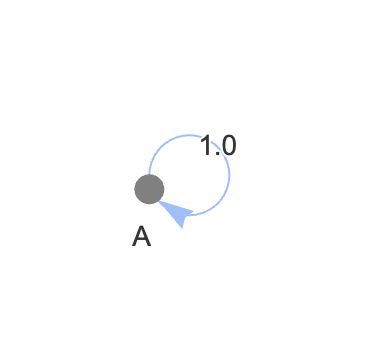
\includegraphics[width=\textwidth]{invalid_graph_1}
    \end{subfigure}
    \hfill
    \begin{subfigure}[t]{0.32\textwidth}
        \centering
        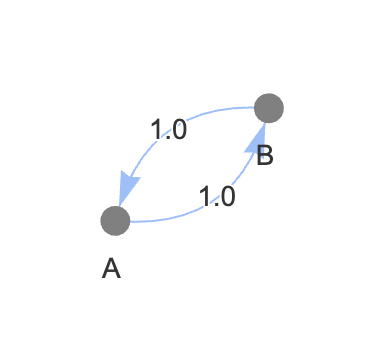
\includegraphics[width=\textwidth]{invalid_graph_2}
    \end{subfigure}
    \hfill
    \begin{subfigure}[t]{0.32\textwidth}
        \centering
        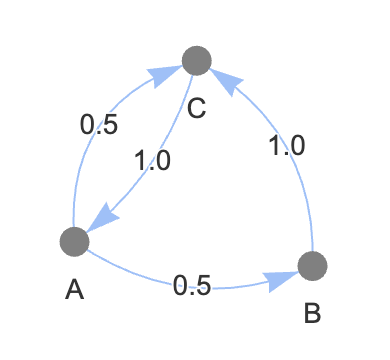
\includegraphics[width=\textwidth]{invalid_graph_3}
    \end{subfigure}
    \caption{Closed delegation cycles}
    \label{fig:closed-delegation-cycles}
\end{figure}

\Cref{fig:closed-delegation-cycles} shows exemplary closed delegation cycles. These cycles lead to contradictory situations, as power delegated within never reaches a sink. Some works discuss ways to handle power stuck in such cycles or mitigate the risk of such cycles appearing, but effectively it is lost. \cite{behrensCircularDelegationsMyth2015, brillInteractiveDemocracy2018} This means that none of the nodes in a closed cycle will vote, which is in line with the will of voters, who all wish to not vote themselves, instead delegate their power, letting their delegate(s) decide what to do with this power. 

In practice, such cycles need to be addressed before resolving delegations in a preprocessing step. Our approach to this is to find all such cycles, and collapse them into an additional sink node in the graph, the \textbf{cycle sink node}. Any delegation into the cycle is redirected into the cycle sink node,  thus ensuring the graph no longer has any closed delegation cycles. The algorithm to do so can be found in annex XX. \TODO{Add this into the annex, if that necessary...} 

We prove below, that given the absence of such closed delegation cycles, delegations are resolvable given a delegation graph. 

\begin{theorem}
Let $G = (S \dot\bigcup D, E)$ be a delegation graph. If $G$ contains no closed delegation cycles, then for every delegator $d \in D$, there exists a path from $d$ to a sink node $s \in S$.
\end{theorem}
\begin{proof}
Suppose, for contradiction, that $G$ contains no closed delegation cycle, but $\exists d \in D$ such that no path from $d$ leads to any sink $s \in S$. Since G is a finite graph, any walk from $d$ must eventually repeat nodes, implying a cycle. If at least one node in this cycle can reach a sink, there would be a path for all others in the cycle to reach a sink via this node as well, thus all nodes in the cycle can not reach a sink either. Thus, G does contain a closed delegation cycle. $\lightning$
\end{proof}

We define a \textbf{well-formed delegation graph} as a delegation graph, which contains no closed delegation cycles. Note, that while a self loop of weight one is not allowed in a well-formed delegation graph, a self loop of weight $w < 1$ is allowed as long as the rest of the node's power eventually flows to a sink. Since a delegator cannot vote themselves, any power it delegates to itself will "flow" back into the node, and then be redistributed to its delegates. 

\section{Resolving Delegations}
\label{sec:resolving_delegations}

\begin{figure}[t]
	\centering
	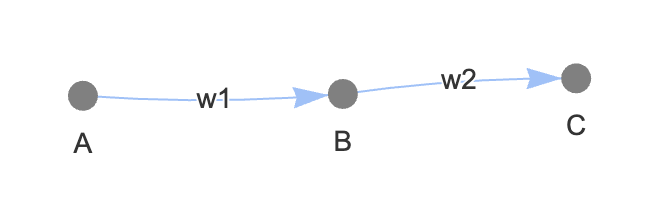
\includegraphics[width=0.4\textwidth]{delegation_graph_sample}
	\caption{Sample delegations}
	\label{fig:sample_delegations}
\end{figure}

We will use the sample delegation chain in \cref{fig:sample_delegations} to create an intuition on how we will resolve delegation graphs. Sink node $C$ receives its own initial vote, and is also delegated a fraction $w_2$ of $B$'s vote. Node $B$, in turn, receives its own vote and a fraction $w_1$ of A's vote. Let $p'_A$ and$ p'_B$ denote the \textbf{standing power} of nodes $A$ and $B$, i.e. the total amount of power delegated to them. Then, the final power of $C$, assuming no other incoming delegations, is:

\begin{align*}
p_C &= 1 + w_2p'_B \\
&= 1 + w_2(1 + w_1p'_A) \\
&= 1 + w_2(1 + w_1 \cdot 1)
\end{align*}

This motivates the recursive definition of standing power in a delegation graph $G = (V, E)$ as:

\[
p'_v = 1 + \sum_{(u, v, w) \in E} wp'_u
\]

Using this definition, and in line with the problem statement that delegating nodes must not retain any power, we define the final voting power $p_v$ of a node as:
\[
p_v = 
\begin{cases}
p'_v & \text{if } v \in S \\
0     & \text{if } v \in D
\end{cases}
\]

The problem of finding each node's standing power is thus a problem of solving a system of linear equations, namely calculating the standing power for all nodes. We can prove, that given a well-formed delegation graph, this method returns a unique solution, and power is conserved.

\subsection{Existence of a Unique Solution}
\label{subsec:unique_sol}

The system of linear equations $p'_v = 1 + \sum_{(u, v, w) \in E} wp'_u$ can also be rearranged to be in matrix form: 

\begin{align*}
p' = \mathbb{1} + Wp' &\implies p' - Wp' = \mathbb{1} \\
&\implies (I - W)p' = \mathbb{1}
\end{align*}

where \( p' \in \mathbb{R}_+^{|V|} \) is the vector of standing power values for each node, \( W \in (0, 1]^{|V| \times |V|} \) is the adjacency matrix of the graph (with \( W_{ij} \) denoting the weight of the edge from node \( j \) to node \( i \)), and \( \mathbb{1} \) is the all-ones vector. This notation will be used within the proof below.

\begin{theorem}
Given a well-formed delegation graph $G=(V, E)$, the equation $p'_v = 1 + \sum_{(u, v, w) \in E} wp'_u$ has a unique solution for all $v \in V$.
\end{theorem}
\begin{proof}

The theorem holds trivially if $|V| = 0$, since the statement “for all $v \in V$” is vacuously true.

Assume now that $G = (V, E)$ contains at least one node. Let $G' = (V, E')$, where
\[
E' = E \cup \{(s, s, 1) \mid s \text{ is a sink in } V\}.
\]
By construction, each node in $G'$ has outgoing edges whose weights sum to 1, so $G'$ is a (row-stochastic) Markov chain. Furthermore, $G$ satisfies the following:

\begin{enumerate}
\item There exists at least one sink (follows from well-formedness and $|V| > 0$),
\item Every node has a path to at least one sink (by assumption on well-formed delegation graphs).
\end{enumerate}

Thus, $G'$ is an absorbing Markov chain: every state can reach an absorbing state (a sink with a self loop) in finite steps. A standard result for such chains is that their transition matrix $P$ can be rearranged as:

\[
P = \begin{bmatrix}
Q & R \\
0 & I_r
\end{bmatrix},
\]

where $Q$ describes transitions between transient (non-sink) states, $R$ transitions from transient to absorbing states, and $I_r$, the identity matrix, the transitions from absorbing states, which necessarily always transition back into themselves. After infinite transitions, the probability of still being in a transient state is zero, thus $\lim_{k \to \infty} Q^k = 0$, which implies that $Q$'s spectral radius $\rho(Q) < 1$.

Now consider the system of linear equations

\[
(I - W)p' = \mathbb{1}
\]

Let $W^T$ be $W$'s transpose. Then $W^T$ structurally resembles a transition matrix, with row sums = 1.

Define the subgraph $D \subset G$ induced by all delegating (non-sink) nodes. Let $W_D^T$ be the transpose of the weight matrix for $D$, which only includes delegations among delegating nodes. 

Then $W_D^T = Q$, so $W_D = Q^T$ and $\rho(W_D) = \rho(Q) < 1$. The equality of the two matrices follows from the observation that the construction of $G'$ from $G$ only adds self-loops to sink nodes, leaving all delegating nodes and their outgoing edges unchanged.

Note that standing power values for delegating nodes depend only on the values of other delegators — never on sink nodes. This justifies restricting the analysis to the submatrix $W_D$, as the equation system governing these nodes is self-contained.

We now restrict our attention to the system of equations over only the transient nodes:
\[
(I - W_D) p'_D = \mathbb{1}.
\]

Since $\rho(W_D) < 1$, the Neumann series
\[
(I - W_D)^{-1} = \sum_{k=0}^{\infty} W_D^k
\]
converges, and thus $(I - W_D)$ is invertible. Therefore, $p'_D$ has a unique solution.

Finally, since the standing power of each sink depends only on the standing power values of delegators, and those are uniquely determined, the full vector $p'$ is uniquely determined as well.
\end{proof}

 \subsection{Conservation of Power}
 
 In order to assure that the power is conserved during delegation, it may seem intuitive to add a constraint $\sum_{s \in S} p_s = |V|$ to the system of linear equations. However, we prove that such an equation is not necessary, as the other equations in the system of equations already imply the conservation of power.

We start with the solutions $\{p'_v | v \in V\}$.

Summing over all $v \in V$:
\begin{align*}
\sum_{v \in V} p'v &= \sum_{v \in V} \left( 1 + \sum_{(u, v, w) \in E} wp'_u \right) \\
&= |V| + \sum_{(u, v, w) \in E} wp'_u \numberthis \label{eq:cons_1}
\end{align*}

Now regroup the second term by the source node $u$:

\begin{align*}
\sum_{(u, v, w) \in E} wp'_u &= \sum_{u \in V} \sum_{(u, v, w) \in E} wp'_u  \\ 
&= \sum_{u \in V} p'_u  \sum_{(u, v, w) \in E} w \\
\intertext{
According to our definition of a delegation graph, all sinks have no outgoing notes, and all delegators's outgoing node weights add up to 1. So, for any node $u$::
\[
\sum_{(u, v, w) \in E} w = \begin{cases} 1, u \in D \\ 0, u \in S \end{cases}
\]
Thus we can split the outer sum:
} 
&= \left(\sum_{u \in D} p'_u  \sum_{(u, v, w) \in E} w \right) + \left( \sum_{u \in S} p'_u  \sum_{(u, v, w) \in E} w \right) \\
&= \left( \sum_{u \in D} p'_u \cdot 1 \right) + \left(\sum_{u \in S} p'_u \cdot 0 \right) \\
&= \sum_{u \in D} p'_u \numberthis \label{eq:cons_2}
\end{align*}


At the same time, $V = S \bigcup D$ , and $S$ and $D$ are disjunct, we can split the term $\sum_{v \in V} p'_v$ into:

\[
\sum_{v \in V} p'_v = \sum_{v \in S} p'_v  + \sum_{v \in D} p'_v \numberthis \label{eq:cons_3}
\]

Therefore, combining \eqref{eq:cons_2} and \eqref{eq:cons_3}, the original equality \eqref{eq:cons_1} turns into:

\begin{align*}
\sum_{v \in S} p'_v  + \sum_{v \in D} p'_v &= |V| + \sum_{u \in D} p'_u \\
\implies \sum_{v \in S} p'_v  &= |V| \qed
\end{align*}

\subsection{Resolving Delegations by Solving a System of Linear Equations}

With the insights gained in the previous sections in mind, it is now possible to formulate the following method to resolving delegation graphs.

\begin{enumerate}
\item Set up a system of linear equations, such that for each node $v \in V$ there is an equation $p'_v = 1+\sum_{(u, v, w) \in E}wp'_u$
\item Solve the system of linear equations to find the value of $p'_v$ for all $v \in V$
\item For each $s \in S$ set $p_s = p'_s$
\item For each $d \in D$ set $p_d = 0$
\end{enumerate}


% !TEX root = thesis.tex
\graphicspath{{./figures/}}

%%%%%%%%%%%%%%%%%%%%%%%%
\chapter{Implementation}
%%%%%%%%%%%%%%%%%%%%%%%%

The design above allows for multiple implementations, which will be introduced in this section. This section will also discuss briefly the robustness of the implementations, meaning how they respond to invalid input graphs. They will be explored and evaluated in section XX. Specifically, this paper will cover three implementations, which were chosen as they promise efficiency and scalability.

The implementations were coded in Python. Python is versatile, simple, and offers a large collection of helpful libraries like NetworkX, a library for working with graphs \cite{hagbergExploringNetworkStructure2008}. 

The algorithms take as input python dictionaries ("dicts"), as inputs, which map a key to a value \cite{pythonsoftwarefoundationPythonTutorialSection}. The delegation graph is represented in a "dict of dicts" format, where every key in the outer dict is a node, and the value is another dict, which has the node's neighbors as keys, and a weight as value. The algorithm's use as input "inverse" delegation graphs, where the inner dictionaries represent a node's incoming delegations rather than its outgoing edges. \Cref{fig:inverse_dict_example} shows an example of this. Considering that the standing power equations used in the system of linear equations list contain the incoming delegations for each node, this design choice improves efficiency as an algorithm can look up a node in the dictionary and learn about all its incoming delegations.

\begin{figure}[t]
    \centering
    \begin{subfigure}[t]{0.45\textwidth}
        \centering
        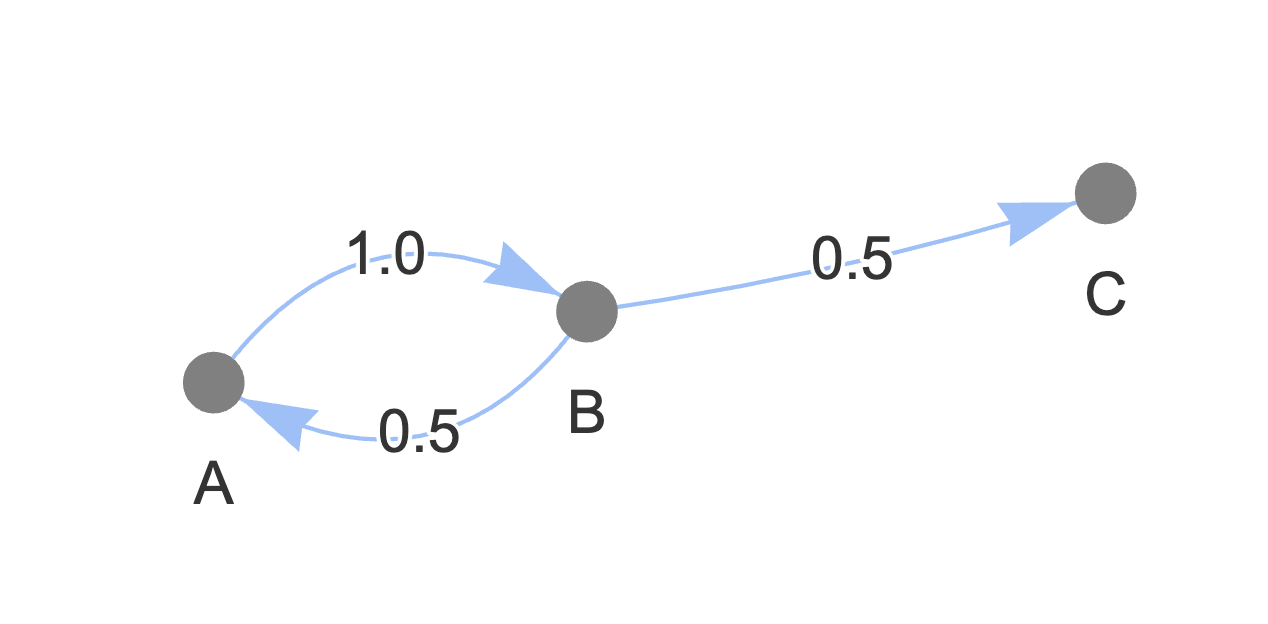
\includegraphics[width=\textwidth]{small_cycle_graph}
        \caption{Delegation graph}
    \end{subfigure}
    \hfill
    \begin{subfigure}[t]{0.45\textwidth}
        \centering
        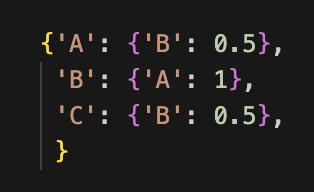
\includegraphics[width=\textwidth]{small_cycle_graph_inverse_dict}
        \caption{Inverse dict representation}
    \end{subfigure}
    \caption{Delegation graph and its inverse dict representation}
    \label{fig:inverse_dict_example}
\end{figure}

\section{Linear System Solver (LS)}

The first approach uses a dedicated linear system solver. We use SciPy's \texttt{scipy.sparse.linalg.spsolve} solver, which is optimized for sparse matrices \cite{virtanenSciPy10Fundamental2020}. A sparse solver is better equipped to resolve delegations if we assume that realistically each delegator only delegates to a few delegates. Since each $wp_v$ term in the system of linear equations can be mapped to one unique edge $(u, v, p) \in E$, the matrix corresponding to the system of linear equations likely has relatively few non zero entries compared to its size. In other words:

\[
\text{For a small } n \in \mathbb{N} \text{, and a large |V|}, D \subset V: n \cdot |D| < |V| \cdot |V|
\]

 \TODO{This explanation is ugly, but idk if its worth spending a lot more time on...} 
 
 The implementation makes use of SciPy's Compressed Sparse Column (CSC) arrays, which builds matrixes using $(x,y)$ coordinates and their corresponding data, which unless specified otherwise is 0 \cite{virtanenSciPy10Fundamental2020}. 

\TODO{This sentence below abt the perfect accuracy makes no sense atm, change it to fit into this section}
The solver solves the system of linear equations directly, using the SuperLU solver, so it is not possible to trade off runtime for accuracy, as done in the previous methods \cite{liSuperLUUsersGuide1999}. 

\section{Linear Programing Solver (LP)}

Secondly, we use the Python library PuLP, which provides an interface to Linear Programming (LP) solvers \cite{osullivanPuLPLinearProgramming2011}. To resolve the delegation graphs, we use the "Coin-or branch and cut" (CBC) solver, since it is free and open-source \cite{johnforrestCoinorCbcRelease2024}. Given the academic context and the moderate size of our delegation graphs, CBC provides a practical balance between performance and accessibility. Moreover, since our model essentially solves a system of linear equations with a unique correct solution, the choice of solver has little influence on the outcome itself — even if CBC is not the most optimized solver for this class of problems. While commercial solvers may offer faster runtimes, CBC is sufficient for our use case and ensures reproducibility without licensing constraints.

\TODO{The mention below abt the perfect accuracy makes no sense atm, since we have not introduced the iterative solver yet, change it to fit into this section}
The algorithm first sets up the linear program, setting up an equation $p'_v = \sum_{(u, v, w) \in E} 1 + wp'_u$ for each node $v \in V$. This is then solved by the CBC solver, with the primal tolerance set to $5*10^{-3}$ to level the playing field compared to the iterative algorithm, which does not have perfect accuracy either. A tolerance of $5 * 10^{-3}$ assures that $\lvert p'_v -\sum_{(u, v, w) \in E} 1 + wp'_u \rvert \le 5*10^{-3}$, so the solutions will be correct when rounded to the second decimal place \cite{forrestCBCUserGuide2005}. Finally, the algorithm cleans the $p_v'$ values, setting any delegators power to 0. 


\TODO{Add links to the implementations on GitHub}

\section{Iterative Solver (Iterative)}

The iterative solver aims to leverage the format of the input, and eliminate any necessary overhead. It is based on the Jacobi method of solving systems of linear equations, which solves the system by iteratively refining the solution \TODO{cite}, however we will prioritize an intuitive explanation of the procedure.

\subsection{Approach}

A delegation can be thought about as liquid throwing through a graph. Each delegator is a "source", and power flows from its source between nodes until it eventually ends in a sink. If a delegator A delegates half their vote to B and the other half to other nodes, half of A's power should flow to B. An algorithm should thus add 0.5 to Bs power, and remove it from A. If B is a sink, the algorithm is done resolving this delegation. However,  B may not be a sink, in which case, the power continues to flow further, to B's delegates. An algorithm would need to iterate over the graph multiple times, until an equilibrium has been reached, where all power in the graph has flown into a sink. \Cref{alg:iterative_simple} shows such an algorithm drafted in pseudocode. Each iteration, a snapshot of the power's of each node is taken, and the reassignments of power are based on this snapshot\footnotemark.  

\footnotetext{If the algorithm forwent the use of such a snapshot, it would lead to inconsistencies in the edge case of a self-delegation of weight less than 1, since the self-delegator's power would change in the middle of reassigning the power. This is also how the Jacobi method approaches this challenge. Each iteration, a solution vector containing intermediate results is created, and passed as input into the next iteration.}

Another valid approach would be a queue-approach, where the algorithm pops node off a queue and delegates their power, and each delegate of this node gets re-added to the queue. A sweeping method treating the entire graph at once was chosen due to its increased simplicity and runtime analysis.

\begin{algorithm} [H]
 \caption{Iterative Algorithm}\label{alg:iterative_simple}
\begin{algorithmic}[1]
\State // Initialize each node’s power to 1.0  
\ForAll{\(v \in \texttt{nodes}\)}
    \State \(\texttt{powers}[v] \gets 1.0\)
\EndFor
\Repeat
    \State \(\texttt{prev\_powers} \gets \texttt{powers}.\texttt{copy}()\)  \Comment{snapshot of previous iteration}
    \ForAll{\(v \in \texttt{nodes}\)}
        \State // For each incoming delegation \((u \to v)\), move \(w_{uv}\times\) previous power of u
        \ForAll{\((u, w) \in \texttt{delegations}[v]\)}
            \State \(\delta \gets w \times \texttt{prev\_powers}[u]\) \label{alg:iterative_simple_delta_assignment}
            \State \(\texttt{powers}[u] \;-\!=\; \delta\) \label{alg:iterative_simple_remove_delta}
            \State \(\texttt{powers}[v] \;+\!=\; \delta\) \label{alg:iterative_simple_add_delta}
        \EndFor
    \EndFor
\Until{\(\texttt{prev\_powers} = \texttt{powers}\)} \label{alg:iterative_simple_termination_cond}\Comment{a steady state has been reached}
\end{algorithmic}
\end{algorithm}

The following notation will be used throughout the next sections.

$G = (V, E)$ is a well-formed delegation graph, with $V = D \dot\bigcup S$, where D is the set of delegators and S is the set of sinks.

Let $p_v^{(i)}, i \in \mathbb{N}_0$ be \texttt{powers}[v] after the $i$-th iteration of the repeat-until loop, with $p_v^{(0)}$ being the initial power of a node before the first iteration has started. Using this notation, our termination condition for the repeat-until loop at \cref{alg:iterative_simple_termination_cond} of \cref{alg:iterative_simple} is: $\forall v \in V: p_v^{(i-1)} = p_v^{(i)}$

Let $P_D^{(i)} = \sum_{d \in D} p_d^{(i)}$ and $P_S^{(i)} = \sum_{s \in S} p_s^{(i)}$ be the sums of all delegators and all sinks after each iteration.

Let $\delta_{(u, v, w)}^{(i)} = w * p_v^{(i)}$ be the delta assigned in \cref{alg:iterative_simple} at \cref{alg:iterative_simple_delta_assignment} during the $i$th iteration.


\subsection{Conservation of Power}

We show, that this algorithm conserves power throughout iterations. This insight .... XXX \TODO{here}

\begin{theorem}
\label{theo:iterative_cons_of_power}
Given a well-formed delegation graph, in \cref{alg:iterative_simple}, $P_t^{(i)} = P_D^{(i)} + P_S^{(i)}$ is equal to $|V|$ for any $i \in \mathbb{N}_0$.
\end{theorem}
\begin{proof}

We prove the theorem inductively. When $i = 0$ (before the first iteration), each node is assigned a power of 1. So 

\[
\forall v \in V: p_v^{(i)} = 1 \implies P_t^{(0)} = |V|
\]

Assume that for a $k \in \mathbb{N}_0: P_t^{(k)} = |V|$. During iteration $k+1$, the algorithm will iterate over all delegations, and for each $(u, v, w) \in E$, it will remove some $\delta_{(u, v, w)}^{(k+1)}$ from node \texttt{u} in \cref{alg:iterative_simple_remove_delta}, but add this same amount to node \texttt{v} in \cref{alg:iterative_simple_add_delta}. Since the delegation graph is well formed, the outgoing weights of any delegator add up to 1, so for all delegators $u \in D$, the total amount of power they delegate away during iteration $k+1$ adds up to the power they held in iteration $k$.

\begin{align*}
\sum_{(u, v, w) \in E} \delta_{(u, v, w)}^{(k+1)} &=  \sum_{(u, v, w) \in E} wp_u^{(k)} \\
&= p_u^{(k)}  \sum_{(u, v, w) \in E} w \\
&= p_u^{(k)} \cdot 1 \\
&= p_u^{(k)}
\end{align*}

Thus, throughout the iteration of the outer loop, any delegator $u$ only ever moves power it already has, and for each "moving around" of power, conservation is guaranteed since any power subtracted from a delegator is re-added to the delegate. This means that power is only ever moved around, but not lost, and $P_t^{(k+1)} = |V|$. 

By the principles of induction, the assumption holds for any $i \in \mathbb{N}_0$
\end{proof}

\subsubsection{Similarity to the Previous Approach}

Observing the algorithm reveals that the same equations used in the previous approach to resolve delegations can be re-found here. Algorithm starts with a vector of ones, indicating an initial power of each node of one. Furthermore, each iteration, each node $u \in V$ gains power amounting to $\sum_{(u, v, w) \in E} \delta^{(i)}_{(u, v, w)}$. This term can be rearranged as follows:

\begin{align*}
p_v^{(i)} &+= \sum_{(u, v, w) \in E} \delta^{(i)}_{(u, v, w)} \\
&+= \sum_{(u, v, w) \in E} wp_v^{(i-1)}
\end{align*}

Since power is conserved, the same amount is also removed from the node, thus we can say, that

\[
p_v^{(i)} = \sum_{(u, v, w) \in E} wp_v^{(i-1)} \forall v \in V
\]


This is the same al the standing power assigned to all nodes in the previous approach. ($p'_v = 1 + \sum_{(u, v, w) \in E} wp'_u$). Thus, this algorithm solves the same problem as the system of linear equations introduced in the previous section. 

\TODO{This section may still be missing an explanation of the jacobi method. I proved that each iteration I resolve something resembling the initial system of linear equations method, but since the reader does not know the jacobi method, they might not be able to notice the similarity.}

\subsubsection{Implementation}

This section will show, that the algorithm does not necessarily terminate despite input with a well formed delegation graph, after which we propose an amended algorithm.

First, we prove that a sink's power can't shrink, since there is no outgoing edge going out of a sink.

\begin{lemma}\label{lem:sink_non_shrink}
$\forall s \in S: p_s^{(i)} \ge p_s^{(i-1)}$ 
\end{lemma}
\begin{proof}
Assume $p_s^{(i)} < p_s^{(i-1)}$. The power that left $s$ needs to have gone somewhere, since the algorithm conserves power. This implies, that there is a delegation $(s, v, w) \in E$ such that $\exists \delta > 0: \delta \gets w * p_s^{(i-1)}$. This contradicts our definition of a well-formed liquid delegation graph, since any sink can not have any outgoing edges.
\end{proof}

Next, we prove that if a node's power is 0, all its delegator's powers must have been 0 after the previous iteration
\begin{lemma}\label{lem:simple_iterative_empty_node}
$p_v^{(i)} = 0 \implies \forall (u, v, w) \in E: p_u^{(i - 1)} = 0$. 
\end{lemma}
\begin{proof} Assume $p_v^{(i)} = 0$, but $\exists (u, v, w) \in E: p_u^{(i-1)} > 0$

Let $d \in \mathbb{R}_{0}$ be any additional power a node receives, that is not explicitly mentioned.

\[
p_u^{(i-1)} > 0 \implies \delta_{(u, v, w)}^{(i)} > 0 \implies p_v^{(i)} = \delta_{(u, v, w)}^{(i)} + d \implies p_v^{(i)} > 0 \lightning
\]

\end{proof}

Next, we prove that the algorithm terminates at iteration $i+1$ exactly when $P_D^{(i)} = 0$.

\begin{lemma}\label{lem:simple_alg_terminates}
 $p_v^{(i)} = p_v^{(i+1)} \forall v \in V \Leftrightarrow$ $P_D^{(i)} = 0$.
\end{lemma}
\begin{proof}

\begin{align*}
	P_D^{(i)} = 0 
	&\Leftrightarrow p_d^{(i)} = 0, \forall d \in D \\
	&\Leftrightarrow \not\exists (d, v, w) \in E: \delta_{(d, v, w)}^{(i+1)} > 0  &&\text{($\delta$ of a node with power 0 is 0)}\\
	&\Leftrightarrow p_v^{(i)} = p_v^{(i+1)} \forall v \in V \qed  &&\text{($p_v$ doesn't change if zero is added to it)}
\end{align*}
\end{proof}

\begin{theorem}\label{alg:iterative_alg_doesnt_terminate}
Given a well-formed delegation graph, \cref{alg:iterative_simple} may not terminate.
\end{theorem}
\begin{proof} Assume the algorithm terminates on a well-formed delegation graph..

Take the following well formed delegation graph $G = (S \dot\bigcup D, E)$with $S =\{C\}$ and $D = \{A, B\}$. B delegates half their vote to A, and half their vote to C, while A delegates its entire vote back to B. Since the algorithm terminates, there must be an $i \in \mathbb{N}$ such that $P_D^{(i)} = 0$. 

\begin{figure}[h]
    \centering
    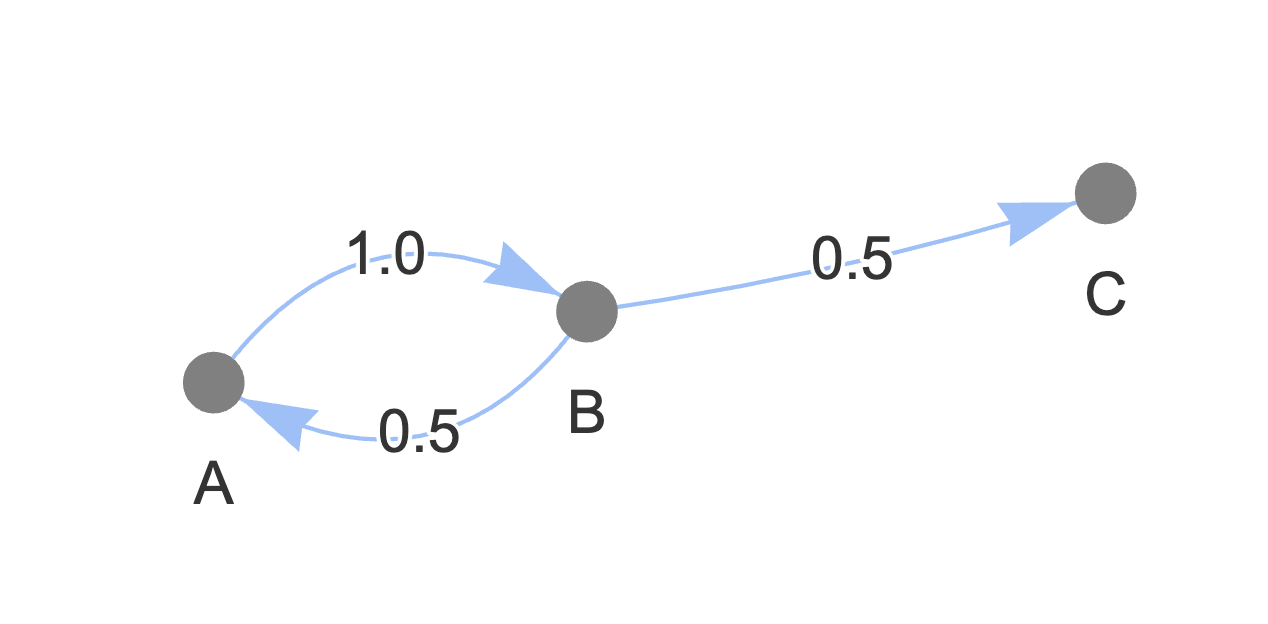
\includegraphics[width=0.4\textwidth]{small_cycle_graph}
    \caption{Delegation graph with a cycle.}
    \label{fig:small_cycle_graph}
\end{figure}


Both (B, A, 0.5) and (A, B, 1) $\in E$, so A is a predecessor of B, and B is a predecessor of A, thus B is its own predecessor.

\begin{align*}
	P_D^{(i)} = 0 
	&\implies p_B^{(i)} = 0 \\
	&\implies p_A^{(i-1)} = 0 &&\text{(Lemma \cref{lem:simple_iterative_empty_node})} \\
	&\implies p_B^{(i-2)} = 0 &&\text{(Lemma \cref{lem:simple_iterative_empty_node})}
\end{align*}

This implication chain can be drawn arbitrarily long. In order for B to have a power of 0, it can never have held any power in the first place, contradicting our well-formed delegation graph, which dictates that all nodes start with a power of 1.
\end{proof}

If the graph is acyclic, this algorithm would need at most $|V|$ iterations, such as in a directed path, where each node gives their entire vote to the next node except for the final sink. However, as soon as cycles are introduced into the graph, the spreading of power only terminates after an infinite amount of steps. Looking further into the graph in \cref{fig:small_cycle_graph}, the expected resolution of these delegations would be that C holds node A and B's powers, as well as its own initial vote, so a power of three. However, looking at the powers as the algorithm iterates over this graph reveals that after the first iteration, C will have 1.5 votes, then 2, then 2.25, 2,50, 2.75, ..., however only after infinitely many steps it will have three. 

\begin{table}[h]
  \centering
  \caption{$p_v{(i)}$ values of nodes in the graph in \cref{fig:small_cycle_graph}}
  \label{tab:simple_iterative_example}
  \begin{tabular}{| l | l | l | l |}
    \hline
    i & $p_A$ & $p_B$ & $p_C $ \\ \hline
    0 & 1 & 1 &	1 \\ \hline
    1 & 0.5 & 1 & 1.5 \\ \hline
    2 & 0.5 & 0.5 & 2 \\ \hline
    3 & 0.25 & 0.5 & 2.25 \\ \hline
    4 & 0.25 & 0.25 & 2.50 \\ \hline
    5 & 0.125 & 0.25 & 2.625 \\ \hline
    \multicolumn{4}{| l |}{...} \\ \hline
  \end{tabular}
\end{table}

Practically, the algorithm needs a cutoff condition, which terminates the while loop once the power values calculated are close enough to the real, final values. Since these are unknown before the algorithm terminates, we can count how much power is being shifted throughout the graph each iteration, and terminate once this value is sufficiently small. An extension to \cref{alg:iterative_simple} could look like \cref{alg:iterative_with_cutoff}. 

\begin{algorithm} [H]
 \caption{Iterative Algorithm with a cuttoff value. Changes from \cref{alg:iterative_simple} are highlighted. }\label{alg:iterative_with_cutoff}
\begin{algorithmic}
\State // Initialize each node’s power to 1.0  
\ForAll{\(v \in \texttt{nodes}\)}
    \State \(\texttt{powers}[v] \gets 1.0\)
\EndFor
\Repeat
    \State \(\texttt{prev\_powers} \gets \texttt{powers}.\texttt{copy}()\) 
    \State \colorbox{yellow}{\(\texttt{total\_change} \gets \texttt{0}\)} 
    \ForAll{\(v \in \texttt{nodes}\)}
        \State // For each incoming delegation \((u \to v)\), move \(w_{uv}\times\) previous power of u
        \ForAll{\((u, w) \in \texttt{delegations}[v]\)}
            \State \(\delta \gets w \times \texttt{prev\_powers}[u]\)
            \State \(\texttt{powers}[v] \;+\!=\; \delta\)
            \State \(\texttt{powers}[u] \;-\!=\; \delta\)
            \State \colorbox{yellow}{\(\texttt{total\_change} \;+\!=\; \delta \)}
        \EndFor
    \EndFor
\Until{\colorbox{yellow}{\(\texttt{total\_change} < \texttt{cutoff}\)}}
\end{algorithmic}
\end{algorithm}

\subsubsection{Conservation of Power}

\Cref{theo:iterative_cons_of_power} states that \cref{alg:iterative_simple} conserves power across iterations. The same proof applies to \cref{alg:iterative_with_cutoff}, since only the if-condition of the outer loop has changed, but the algorithm works the same way. So while the algorithm will iterate less, power remains conserved across iterations.

\subsubsection{Termination}

\begin{lemma}\label{lem:iterative_alg_power_concentrates}
Given a well-formed delegation graph, \cref{alg:iterative_with_cutoff} terminates if \texttt{cutoff} > 0.
\end{lemma}

\TODO{The proof is incomplete, I'll work over it later...}

\begin{proof} We differentiate two cases. Fix an $i \in \mathbb{N}_0$.

Case 1: $P_D^{(i)} = 0$

In this case, no delegator has any power, so the \texttt{total\_change} can be at most 0, which is always smaller than \texttt{cutoff}. So the algorithm terminates.

Case 2: $P_D^{(i)} > 0$

\begin{align*}
P_D^{(i)} > 0 
& \implies \exists d_0 \in D: p_{d_0}^{(i)} > 0 \\ 
& \implies \exists s \in S, \exists k \ge 1, \exists (v_0, ..., v_k): v_0 = d_0, v_k= s, (v_j, v_{(j+1)}, w) \in E \forall 0 \le j \le k \\
&\text{(There is a path between $d_0$ and a sink)} \\
& \implies \exists d_{k-1} \in D: (d_{k-1}, s, w) \in E \\
& \text{($d_{k-1}$ is the node on the path from $d_0$ to $s$ that has an edge to $s$)}
\end{align*}

Assume ${p_{d_{k-1}}}^{(i)} = 0$.

Left $\mathrm{Pred}^*(d_0)$ be defined as follows:

\[
\mathrm{Pred}^*(d_{0})=\bigl\{u \in V \bigm| \exists\text{ a path }u \rightsquigarrow d_{0} \bigr\}
\]

Also, let $\mathrm{dist}(d_{0}, p), p \in V$  be defined as follows :

\[
\mathrm{dist}(d_{0},p) =\min\bigl\{|P| : P\text{ is a path }d_{0}\rightsquigarrow p\bigr\}.
\]

\begin{align*}
{p_{d_{k-1}}}^{(i)} = 0 &\implies 
\end{align*}

$\max\bigl\{\mathrm{dist}(d_0,p)\bigm|p\in \mathrm{Pred}^*(d_0)\bigr\} $

...

%{p_{d_{(k-1)}}}^{(i)} = 0

%The algorithm assumes, that the \texttt{total\_change} eventually shrinks below the cutoff value. 

\TODO{todo continue here, I am too lazy atm to try and figure out how to prove that P\_D shrinks properly}

\end{proof}


\section{Robustness}

This section describes the different implementations behavior when a delegation graph is not well formed. Specifically, their behaviors when outgoing delegation weights are invalid, so not adding up to 1, and if the delegation graph contains a closed delegation cycle. 

\subsection{Invalid delegations}

On their own, neither of the three implementations will definitively cause an error when delegations are invalid. The iterative implementation is "dumb", in the sense that it moves around power as it finds them in the delegations. If a delegator delegates more than they are meant to, the algorithm behavior becomes undefined, since the delegators power may become negative, at which point the delta in power calculated from its power also becomes negative, which messes with the \texttt{total\_change} value in unpredictable ways. 

If a delegate delegates less than their vote, this causes less of an issue. As long as the delta calculated at $\delta \gets w \times \texttt{prev\_powers}[u]$ does not become negative, the algorithm's behavior becomes quite predictable. A well-formed delegation graph is allowed to contain self-delegations as long as their weight is lower than 1, such as the delegation in \cref{subfig:permissible-self-delegation}. In this situation, power still leaves the node, but less slowly. When the iterative algorithm goes over the graph, not delegating enough weight has the same effect as such a self-delegation, since in the former situation  power gets subtracted and then re-added to the node, while in the latter it just remains untouched.

\begin{figure}[h]
    \centering
    \begin{subfigure}[t]{0.45\textwidth}
	\centering
	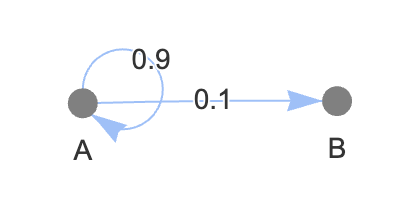
\includegraphics[width=0.9\textwidth]{allowed_self_loop}
	\caption{Permissible delegation graph}
	\label{subfig:permissible-self-delegation}
    \end{subfigure}
    \hfill
    \begin{subfigure}[t]{0.45\textwidth}
        \centering
        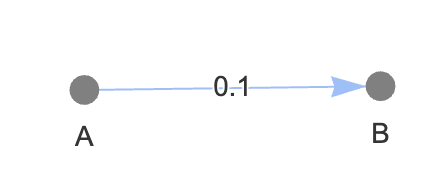
\includegraphics[width=\textwidth]{invalid_delegation_graph}
        \caption{Invalid delegation graph}
         \label{subfig:invalid-delegation-graph} 
    \end{subfigure}
    \caption{Two similar delegation graphs}
    \label{fig:small-delegation-graphs}
\end{figure}

For the two implementations directly based on solving systems of linear equations, this is a little different. Node \texttt{B}'s power would end up as 1.1, since the system of linear equations looks as follows:

\begin{align*}
& p_A = 1 \\
& p_B = 1 + 0.1p_A
\end{align*}

As long as the delegations form a matrix that is singular, there will be a unique solution, so even with invalid delegations, the algorithm will find power values, however they most likely differ whom the power values that would be expected, and probably not conserve total power properly. 

\subsection{Closed Delegation Cycles}

If the delegations form a closed delegation cycle, the iterative algorithm will not terminate, since the algorithm will iterate any power that is in or enters the cycle around the cycle indefinitely. 

For the other two algorithms however, such a cycle can be caught. The equations for the standing power of the nodes within the cycle are linearly dependent on each other, thus the matrix resulting from them is not singular, and hence don't have a single solution. Solvers of systems of linear equations catch and throw an error. Similarly, the LP solver will find that the linear program is infeasible.

What is worth mentioning however, is that since we allow fractional delegation, it suffices if just one node is a closed delegation cycle does also delegates to a node outside of a delegation cycle (or turns into a sink), for the delegations to become resolvable again. The cycles that were explored in \cref{subsec:cycles_draining} are example of such a situation. 



% !TEX root = thesis.tex
\graphicspath{ {./figures/} }

%%%%%%%%%%%%%%%%%%%%
\chapter{Evaluation}
%%%%%%%%%%%%%%%%%%%%

The three algorithms will be evaluated based on their runtime and scalability as well as their robustness, meaning their ability to handle invalid graphs. 

\section{Method}

We will explore the runtime of the algorithms on small graphs, big graphs and then explore their behavior in specific situations and corner cases. For the first two sections, we have built an algorithm, that builds a graph with n nodes, and then adds between zero and three delegations per node to random other nodes, ensuring that there are no delegation cycles without a sink. A better explanation of how these graphs are artificially constructed can be found in the Annex. \TODO{Create this annex} We acknowledge, that these assumptions may not be representative of real delegation graphs, where, as studies have shown, delegates tend to not delegate randomly, but to a subset of experts, such as TV personalities, thus centering power to one or few people. This approach also ignores potential tendencies such as friends delegating to eachother more likely. Such situations will be explored in subsection XX. \TODO{Add citations that these situations happen. Maybe the viscous democracy paper, and the pirate party example, and in one of the six original papers Ford shared this was also mentioned}.

To minimize the impact of background noise and measurement fluctuations on the benchmarks, algorithms with very short runtimes were executed multiple times, and the average runtime was recorded. The recorded runtimes always indicate just the runtime for the algorithms to resolve the delegations, times for set-up, such as the time for building the linear program, were not included. 

\section{Evaluating Runtime and Scalability}

\subsection{Small graphs}
\label{subsec:small_graphs}

\begin{figure}[h]
    \centering
    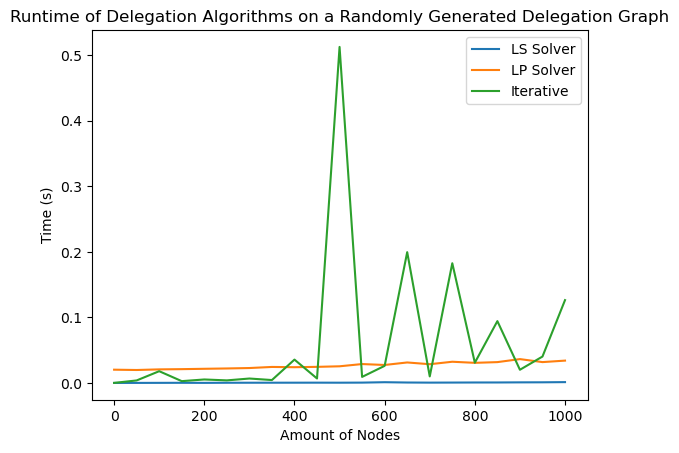
\includegraphics[width=0.4\textwidth]{0-1000_random}
    \caption{Runtime of delegation algorithms on a randomly generated delegation graph.}
    \label{fig:random-small}
\end{figure}

In order to explore the three algorithm's behavior on small graphs, we used the graph generator to generate graphs with zero to 1000 nodes. \Cref{fig:random-small} shows the results of this benchmark.

We can see, that the LS Implementation, optimized for sparse matrices, outperforms the other two algorithms. Its growth in runtime is so small, that the line looks to be staying flat on the x-axis. However, with a graph of 1000 nodes, its runtime is about 0.01 seconds. Both the LS and LP implementation display a rather steady, yet growing runtime. The LP solver seems to have some overhead, since even when the graph has zero nodes, it has a runtime of about 0.02 seconds.

Furthermore, we can interestingly observe large spikes in the runtime of the iterative approach. Exploring this more closely, we find that the graph with 11 nodes takes the iterative algorithm a lot more time than the graph with 10 or 12 nodes, as shown in \cref{fig:random-tiny}. At 10 nodes, the runtime of the iterative algorithm is just about 0.004 seconds, at 12 nodes it is 0.001 seconds, so even slightly faster than the slightly smaller graph, but when the graph has 11 nodes, the runtime skyrockets to about 0.056 seconds.

\begin{figure}[h]
    \centering
    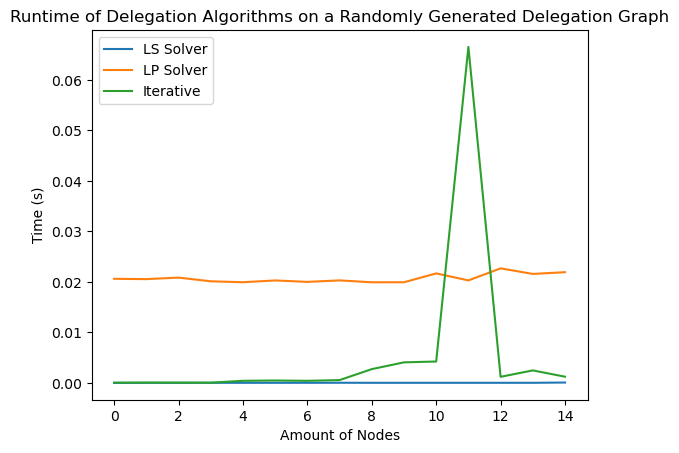
\includegraphics[width=0.4\textwidth]{0-15_random}
    \caption{Runtime of delegation algorithms on a randomly generated delegation graph.}
    \label{fig:random-tiny}
\end{figure}

A possible explanation for this spike may be, that when the graph has 10 and 12 nodes, it iterates only 758 and 170 times respectively, before cutting off, while when it has 11 nodes it iterates 8735 times before cutting off. \Cref{fig:random-11and12} shows the two graphs with 11 and 12 nodes.

\begin{figure}[h]
    \centering
    \begin{subfigure}[t]{0.45\textwidth}
        \centering
        \fbox{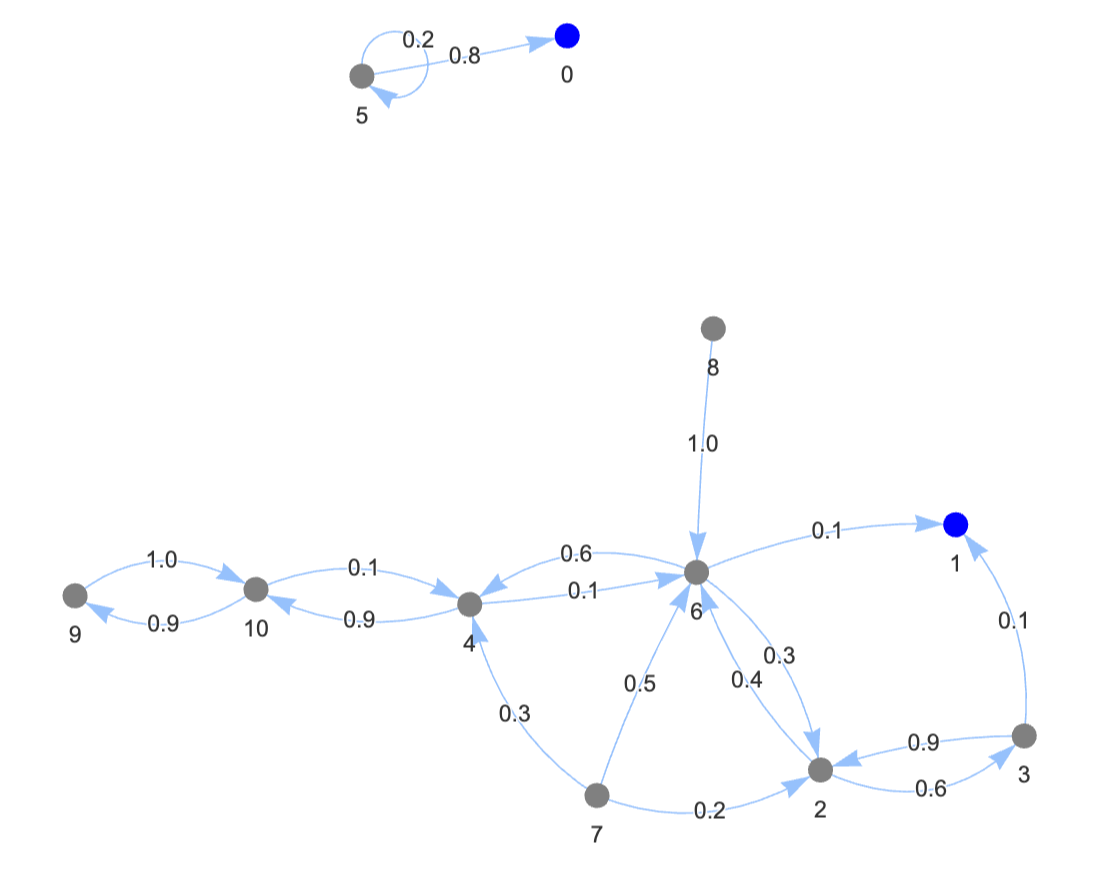
\includegraphics[width=\textwidth]{11_random}}
        \caption{11 nodes}
        \label{subfig:random-11and12-11}
    \end{subfigure}
    \hfill
    \begin{subfigure}[t]{0.45\textwidth}
        \centering
        \fbox{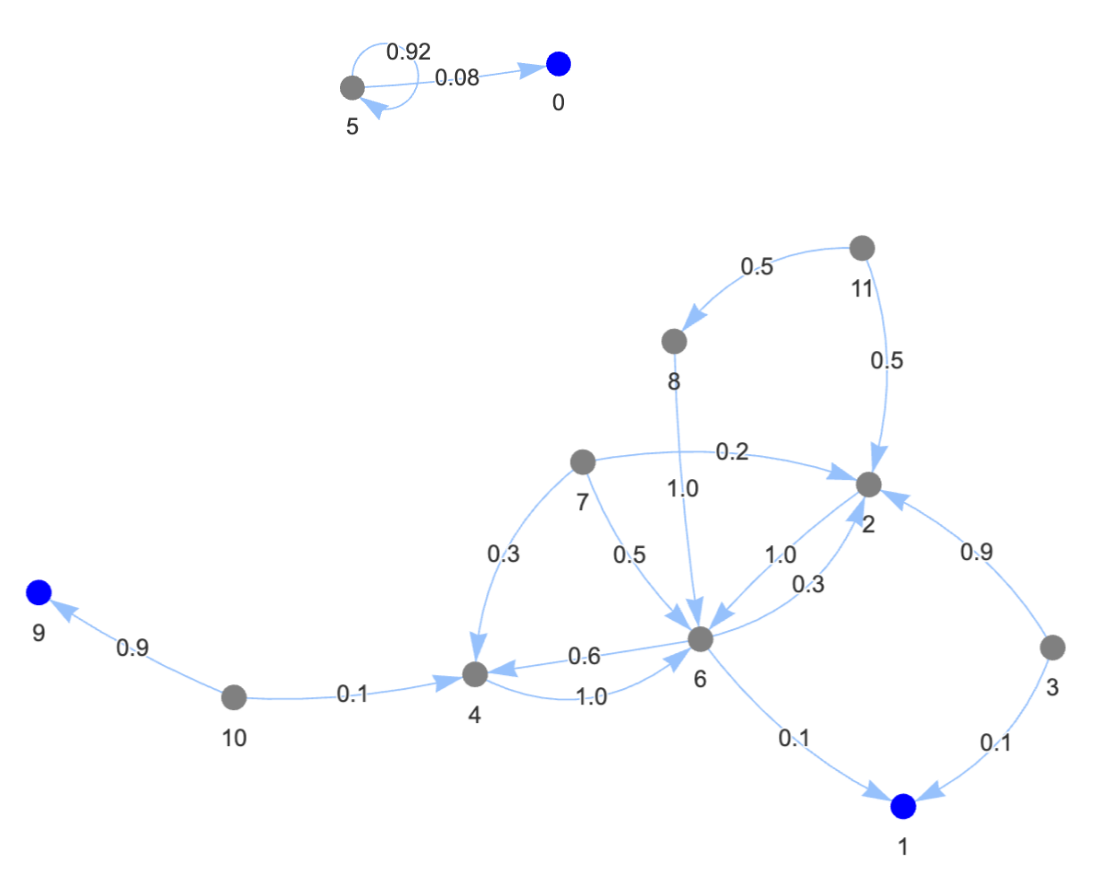
\includegraphics[width=\textwidth]{12_random}}
        \caption{12 nodes}
    \end{subfigure}
    \caption{Delegation graphs with 11 and 12 nodes}
    \label{fig:random-11and12}
\end{figure}

Inspecting the graphs reveals a possible explanation for this behavior. When the graph has 12 nodes, node \texttt{9} is a sink, while in the graph with 11 node it delegates its power back to node \texttt{10}. In the latter case, power going out of node \texttt{9} needs to pass to node \texttt{10}, \texttt{4} and \texttt{6} before reaching a sink. While passing through node \texttt{4}, we can see that 90\% of the power is delegated back into the cycle between nodes \texttt{4}, \texttt{10} and \texttt{9}. The algorithm will iterate power through this loop, until enough has been drained out for the \texttt{total\_change} to fall below the cutoff. 

This is an important shortcoming of the iterative algorithm. Power can easily get trapped within permissible delegation cycles that only have a small drain allowing the power to escape from the cycle. Each iteration, if a great proportion of the nodes with draining edges' power is sent back into a cycle, the algorithm needs to continuously iterate until the power is back at the drain nodes, however depending on the cycle this may happen very inefficiently. This phenomenon will be tested more in \cref{subsec:cycles_draining}

\subsection{Large Graphs}

Delegation graphs may grow arbitrarily large. National elections for example can contains up to hundreds of millions of participants. This section explores how the algorithms perform when having to resolve graphs with a lot of nodes. Again, the graphs will be randomly generated, such that each nodes has between 0 and 3 delegates. 

\begin{figure}[h]
    \centering
    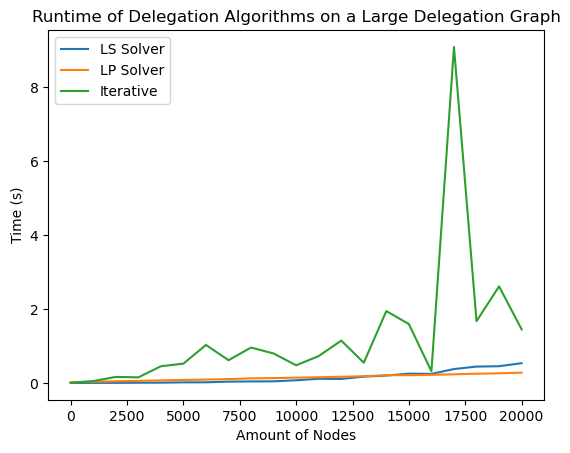
\includegraphics[width=0.4\textwidth]{0-20000_random}
    \caption{Runtime of delegation algorithms on a randomly generated delegation graph.}
    \label{fig:random-large}
\end{figure}

In \cref{fig:random-large} we can see, that it is difficult to determine a pattern in the runtime for the iterative algorithm. Depending on the underlying delegation graph, the runtime can grow unpredictably large. What is evident from the runtime graph however, is that in as the graphs get larger its runtime never subceeds the runtimes of the other two algorithms, while it is worth mentioning that for some graphs, the iterative algorithm's runtime is not a lot longer than that of the other two algorithms. It is difficult to make any statement about the runtime class of the iterative algorithm based just on the number of nodes in the graph, since, depending on the structure of the graph and the cutoff value the runtime can get arbitrarily high. The comparatively high runtime of the iterative algorithm overshadows the runtimes of the other two, so in order to better discuss and analyze their performance, \cref{fig:random-large-no-iterative} shows the same graph as in \cref{fig:random-large}, without the runtimes for the iterative algorithm.

\begin{figure}[h]
    \centering
    \begin{subfigure}[t]{0.45\textwidth}
        \centering
        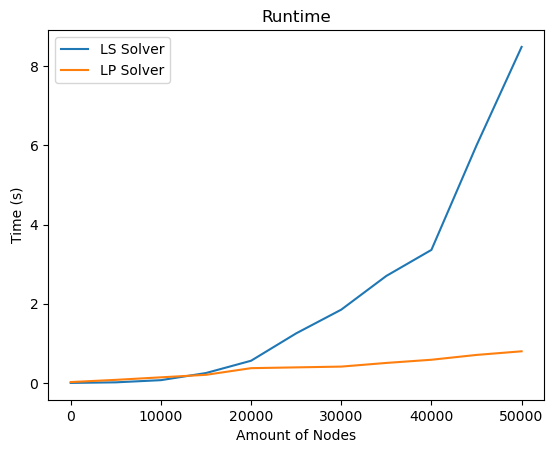
\includegraphics[width=\textwidth]{0-50000_random_no_iterative}
        \caption{Linear scale}
         \label{subfig:random-large-no-iterative-linear}
    \end{subfigure}
    \hfill
    \begin{subfigure}[t]{0.45\textwidth}
        \centering
        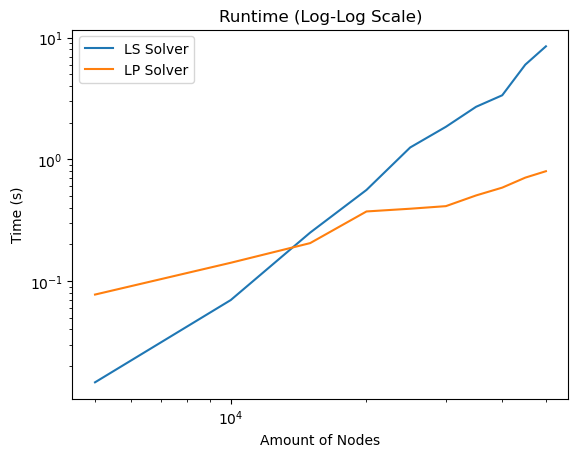
\includegraphics[width=\textwidth]{0-50000_random_no_iterative_loglog}
        \caption{Loglog scale}
         \label{subfig:random-large-no-iterative-loglog}
    \end{subfigure}
    \caption{Runtime of delegation algorithms on a randomly generated delegation graph.}
    \label{fig:random-large-no-iterative}
\end{figure}

\begin{figure}[h]
    \centering
    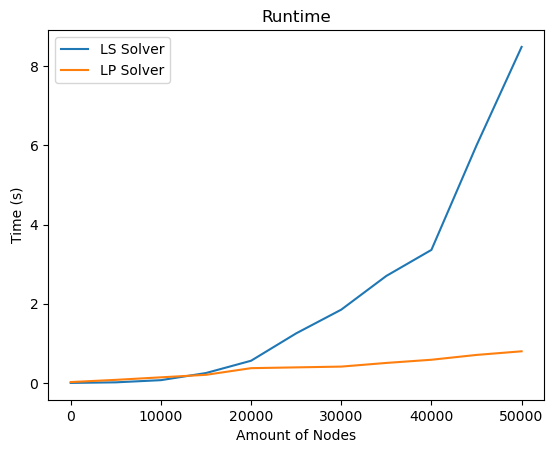
\includegraphics[width=0.4\textwidth]{0-50000_random_no_iterative}
    \caption{Runtime of delegation algorithms on a randomly generated delegation graph.}
    \label{fig:random-large-no-iterative}
\end{figure}

\Cref{subfig:random-large-no-iterative-linear} shows, that as the delegation graph grows, the LP solver's runtime grows more slowly than the LS Solver's. For resolving smaller graphs, the LS solver outperforms the LP solver, with a runtime of almost zero for empty or very small graphs, while the LP solver has a clearly non-zero runtime even for very small graphs. However, at around 12 000 nodes, this changes, as the LP solver's runtime's slower growth catches up with that of the LS solver. 

The type of growth, so the runtime class, is not immediately clear from the graphs, although the LP solver's growth seems to be more linear than that of the LS solver. Looking at the same results on a loglog graph reveals, that the LS solvers runtime may follow a power law.

Fitting the data into different kinds of curves reveals, that the LP implementations runtime likely has linear growth, while the LS solver grows following a power distribution, such that it is in the runtime class of $O(n^{2.778})$.

\TODO{Put the runtime results and/or the code and the regression results into the annex, or into the text...}

\subsection{Dense Graphs}

While we expect most delegators in any delegation graph to only delegate to a handful of people, a well formed delegation graph can have any number of delegates per delegator. Thus, it is also interesting to compare how the three algorithms compare when resolving more dense graphs. In this section, we test the three implementations on NetworkX's $G_{n,p}$ graph generator \texttt{gnp\_random\_graph}, which returns a directed graph with $n$ nodes, where each node connected to each other node with probability $p$, which is set to $0.5$ for the remainder of this section.\TODO{Insert missing citation} These graphs are not well-formed delegation graphs out-of-the box, thus we adapt them by removing outgoing edges of nodes, turning them into sinks, until 10\% of the nodes are sinks. Then, each delegators vote is equally distributed to all of its outgoing edges, such that the edge weights add up to 1. Finally, any closed delegation cycles are removed by removing a random edge in the cycle (and re-normalizing the edge weights). 

% \TODO{cite here https://networkx.org/documentation/stable/reference/generated networkx.generators.random_graphs.gnp_random_graph.html} at the end of the sentence where I introduce this graph

\begin{figure}[h]
    \centering
    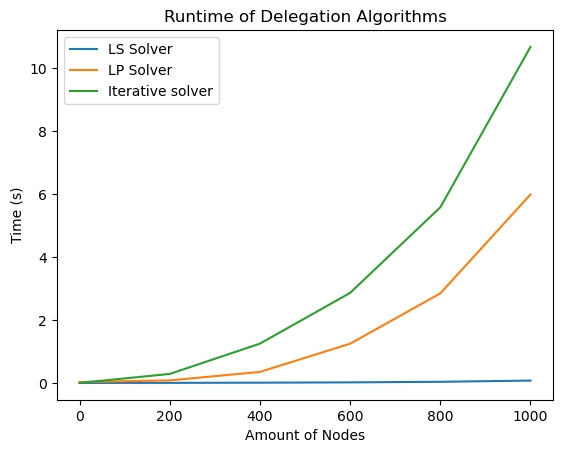
\includegraphics[width=0.4\textwidth]{0-1000_dense}
    \caption{Runtime of delegation algorithms on a randomly generated delegation graph.}
    \label{fig:dense-small}
\end{figure}

\Cref{fig:dense-small} shows the runtime of these three algorithms. The runtime of the iterative algorithm lacks the spikes found when resolving sparse graphs. This is likely due to the nature of the graphs we create. Every delegator is connected to half of all other nodes ($p = 0.5$), and of these $10\%$ are sinks, thus power drains quickly into sinks, and situations where power iterates a long time without seeing a sink are less frequent. Regardless, the iterative algorithm exhibits the worst runtime of the three. 

\begin{figure}[h]
    \centering
    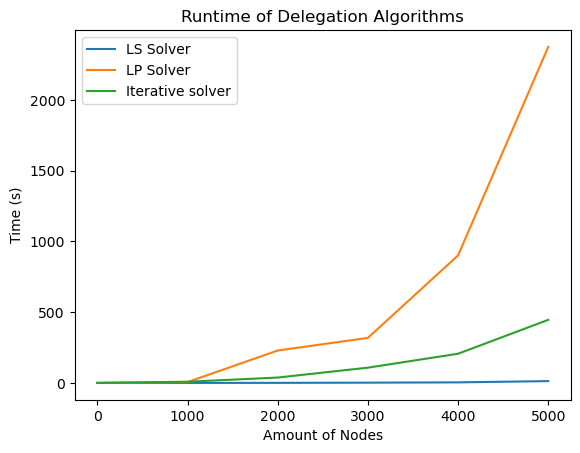
\includegraphics[width=0.4\textwidth]{0-5000_dense}
    \caption{Runtime of delegation algorithms on a randomly generated delegation graph.}
    \label{fig:dense-large}
\end{figure}

Testing the three algorithms on larger dense graphs, reveals surprisingly, that the LP solver's runtime is considerably worse than that of both the iterative and LS solver. A dense graph with 5,000 nodes, and thus about 125,000 delegations, takes the LS solver only about 12 seconds, the iterative solver 445 seconds, and the LP solver almost 2,400 seconds. Even though the LS solver is optimized for sparse matrices, it outperforms the other two implementations on dense graphs.


\subsection{Cycles which Retain a Lot of their Power}
\label{subsec:cycles_draining}

\begin{figure}[h]
	\centering
	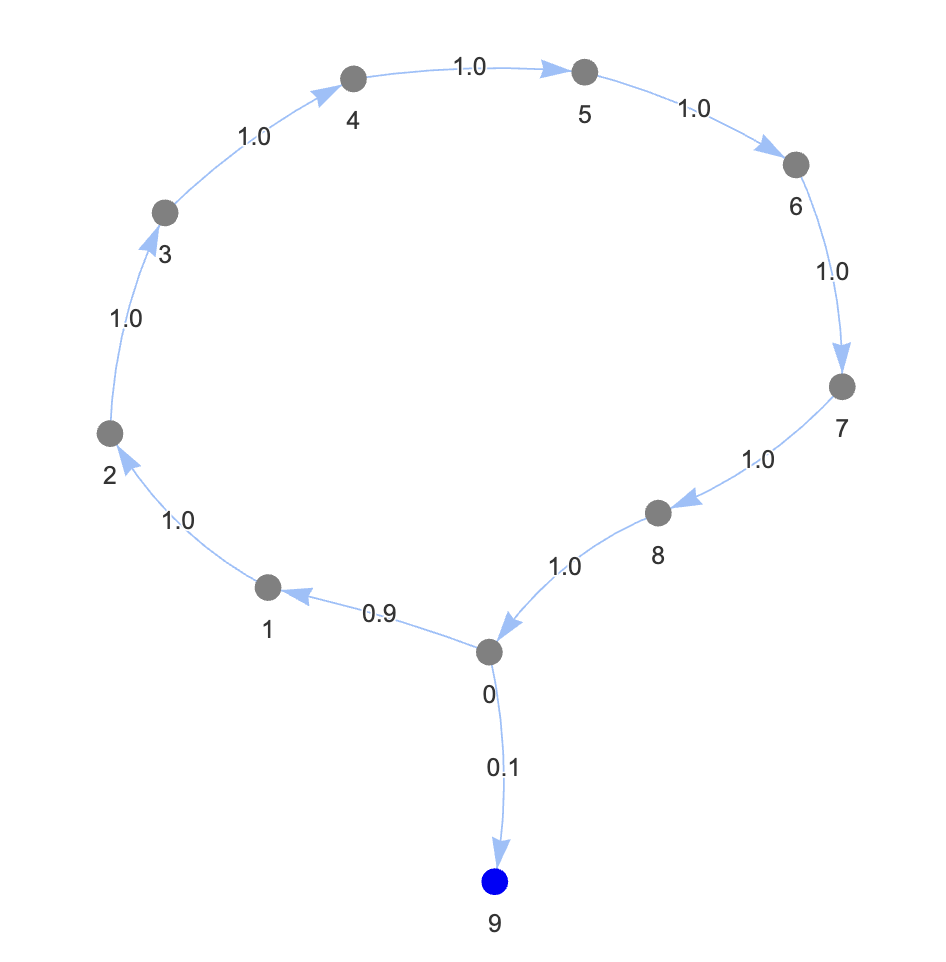
\includegraphics[width=0.4\textwidth]{big_cycle_example}
	\caption{An example of the cycles used for the benchmarks. The blue node is the sink}
	\label{fig:big_cycle_example}
\end{figure}

To further explore one of the iterative algorithm's shortcomings, this section will explore and compare runtime behavior for delegation cycles which are not closed, but contain only few, weak edges for power to drain, thus forcing power to iterate around in the cycle before it reaches a sink. Specifically, we construct graphs with delegates all delegating power to the next node in the cycle. One node in the cycle contains an edge with weight 0.1 to a sink, while the other 0.9 of its power go to the first node in the cycle. \Cref{fig:big_cycle_example} contains an exemplary image of such a graph with 10 nodes. 

\begin{figure}[h]
    \centering
    \begin{subfigure}[t]{0.45\textwidth}
    	\centering
    	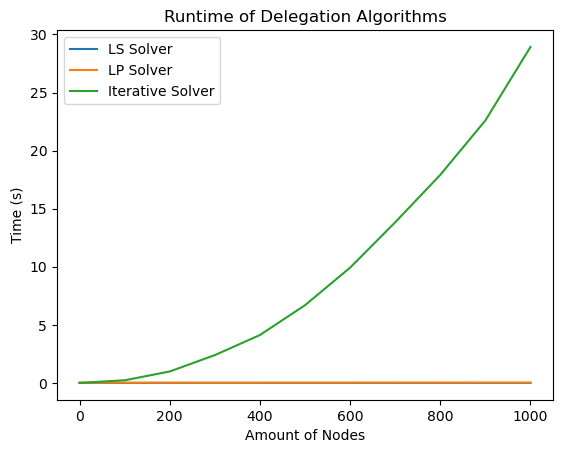
\includegraphics[width=\textwidth]{0-1000_cycle}
    	\caption{Linear scale}
    	\label{subfig:cycle-small-linear}
    \end{subfigure}
    \hfill
    \begin{subfigure}[t]{0.45\textwidth}
        \centering
        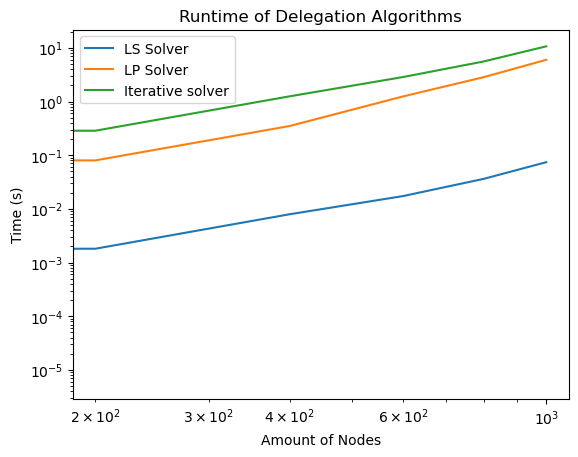
\includegraphics[width=\textwidth]{0-1000_dense_loglog}
        \caption{Loglog scale}
         \label{subfig:cycle-small-loglog}
    \end{subfigure}
    \caption{Runtime of delegation algorithms on a randomly generated delegation graph.}
    \label{fig:cycle_small}
\end{figure}

The runtimes in \cref{subfig:cycle-small-linear} show, that as expected, the iterative algorithm struggles considerably with the resolution of these graphs, while the other two algorithms exhibit behavior similar to that on randomly generated sparse delegation graphs. The growth of the runtimes seems to be polynomial, with the iterative algorithm belonging to the runtime class $O(n^{2.12})$. Being able to resolve these kinds of loops is one of the greatest strength of the two approaches, which don't simulate power as flow through the graph. By directly solving the system of linear equations, they are a lot more well equipped to deal with this specific corner case.  

\begin{figure}[t]
	\centering
    	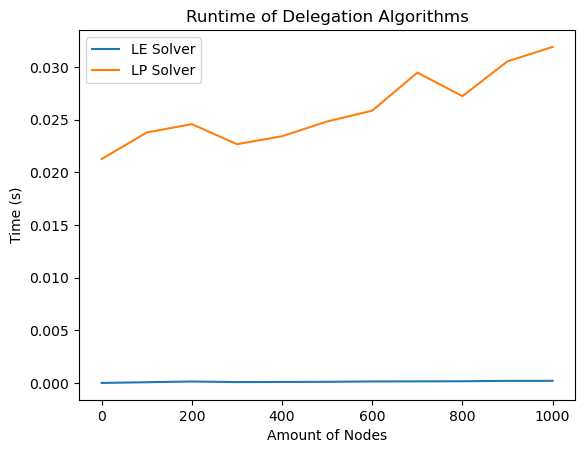
\includegraphics[width=0.4\textwidth]{0-1000_cycle_no_iterative}
    	\caption{Runtime of delegation algorithms on a randomly generated delegation graph.}
	\label{fig:cycle-small-no-iterative-linear}
\end{figure}

As seen in \cref{fig:cycle-small-no-iterative-linear}, which shows the same graph as in \cref{subfig:cycle-small-linear} without the iterative algorithm's runtime, the runtime of the LS and LP Solvers grows similarly to when resolving randomly generated (sparse) delegation graphs, such as the ones found in \cref{subsec:small_graphs}.

Such a cycle as the one we deliberately constructed is not the only situation in which the iterative algorithm will struggle. As long as power is not efficiently funneled toward a sink, the iterative algorithm will have to spend more time moving the power around until enough has drained into a sink for \texttt{total\_change} to fall below the cutoff value. A further example of such behavior is the cycle that caused runtime to spike in \cref{subfig:random-11and12-11}. An artificial example of this situation is shown below in Figure XX. \TODO{Create this graph}


\subsection{Real Example}

So far, we have made use mainly of randomly or artificially generated graphs. This section will briefly confirm, that our insights also hold when resolving delegations based on 

\TODO{I want to try the algorithm on one huge, "real" dataset here}

\TODO{Standord's Large Network Dataset Collection "Epinions" dataset is cool.} 

\TODO{Ill do this later, since while its a cool addition, its probably not going to add a lot of insight thats necessary for the first draft...}


\section{Robustness}

This section the different implementations behavior when a delegation graph is not well formed. Specifically, their behaviors when outgoing delegation weights are invalid, so not adding up to 1, and if the delegation graph contains a closed delegation cycle. 

\subsection{Invalid delegations}

On their own, neither of the three implementations will definitively cause an error when delegations are invalid. The iterative implementation is "dumb", in the sense that it moves around power as it finds them in the delegations. If a delegator delegates more than they are meant to, the algorithm behavior becomes undefined, since the delegators power may become negative, at which point the delta in power calculated from its power also becomes negative, which messes with the \texttt{total\_change} value in unpredictable ways. 

If a delegate delegates less than their vote, this causes less of an issue. As long as the delta calculated at $\delta \gets w \times \texttt{prev\_powers}[u]$ does not become negative, the algorithm's behavior becomes quite predictable. A well-formed delegation graph is allowed to contain self-delegations as long as their weight is lower than 1, such as the delegation in \cref{subfig:permissible-self-delegation}. In this situation, power still leaves the node, but less slowly. When the iterative algorithm goes over the graph, not delegating enough weight has the same effect as such a self-delegation, since in the former situation  power gets subtracted and then re-added to the node, while in the latter it just remains untouched.

\begin{figure}[h]
    \centering
    \begin{subfigure}[t]{0.45\textwidth}
	\centering
	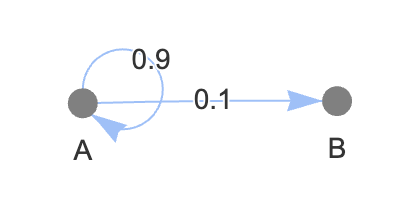
\includegraphics[width=0.9\textwidth]{allowed_self_loop}
	\caption{Permissible delegation graph}
	\label{subfig:permissible-self-delegation}
    \end{subfigure}
    \hfill
    \begin{subfigure}[t]{0.45\textwidth}
        \centering
        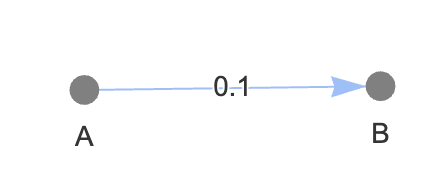
\includegraphics[width=\textwidth]{invalid_delegation_graph}
        \caption{Invalid delegation graph}
         \label{subfig:invalid-delegation-graph}
    \end{subfigure}
    \caption{Two similar delegation graphs}
    \label{fig:small-delegation-graphs}
\end{figure}

For the two implementations based on systems of linear equations, this is a little different. Node \texttt{B}'s power would end up as 1.1, since the system of linear equations looks as follows:

\begin{align*}
& p_A = 1 \\
& p_B = 1 + 0.1p_A
\end{align*}

As long as the delegations form a matrix that is singular, there will be a unique solution, so even with invalid delegations, the algorithm will find power values, however they most likely not conserve power properly. 

\subsection{Closed Delegation Cycles}

If the delegations form a closed delegation cycle, the iterative algorithm will not terminate, since the algorithm will iterate any power that is in or enters the cycle around the cycle indefinitely. 

For the other two algorithms however, such a cycle can be caught. The equations for the standing power of the nodes within the cycle are linearly dependent on each other, thus the matrix resulting from them is not singular, and hence don't have a single solution. Solvers of systems of linear equations catch and throw an error.

What is worth mentioning however, is that since we allow fractional delegation, it suffices if just one node is a closed delegation cycle does also delegates to a node outside of a delegation cycle (or turns into a sink), for the delegations to become resolvable again. The cycles that were explored in \cref{subsec:cycles_draining} are example of such a situation. While closed delegation loops frequently pose a problem in liquid democracies \TODO{cite}, they happen less frequently when allowing fractional delegation \TODO{cite}.



%TODO Maybe mention also at some point, that this evaluation is a comparison between different solvers for systems of linear equations
% !TeX root = ../main.tex

%%%%%%%%%%%%%%%%%%%%%%
\chapter{Related Work}
%%%%%%%%%%%%%%%%%%%%%%

\TODO{Maybe move this up, toward the background section or introduction}

- Degrave paper https://arxiv.org/pdf/1412.4039
	Similar to what we're doing, but they don't consider arbitrary splits of delegations, 
	Propose calculating the final power through systems of linear equations

- Bersetche paper "A Voting Power Measure for Liquid Democracy with Multiple Delegation" \cite{bersetcheGeneralizingLiquidDemocracy2022}
	Here, they propose fractional delegation (called Multiple Delegation)
	Delegates can also retain power for themselves
	Also they propose a penalty factor, in order to XXX

- The Bertsche paper cites some practical experiments with LD, I could include those as well


- The viscous democracy paper might also be relevant

- I remember reading some papers that mention why fractional delegation is benefitial, if it was not the Bersetche paper I'll try to find it again..

% mention here the benefits of fractional delegation
%%%%%%%%%%%%%%%%%%%%
\chapter{Conclusion}
%%%%%%%%%%%%%%%%%%%%

In the conclusion you repeat the main result and finalize the discussion of
your project. Mention the core results and why as well as how your system
advances the status quo.

\cleardoublepage
\phantomsection
\addcontentsline{toc}{chapter}{Bibliography}
\printbibliography

% Appendices are optional
% \appendix
% %%%%%%%%%%%%%%%%%%%%%%%%%%%%%%%%%%%%%%
% \chapter{How to make a transmogrifier}
% %%%%%%%%%%%%%%%%%%%%%%%%%%%%%%%%%%%%%%
%
% In case you ever need an (optional) appendix.
%
% You need the following items:
% \begin{itemize}
% \item A box
% \item Crayons
% \item A self-aware 5-year old
% \end{itemize}

\end{document}